\centering
\begin{subfigure}[b]{0.49\textwidth}
  \centering
  \begin{tikzpicture}[->,shorten >=1pt, node distance={15mm}, main/.style = {draw, circle}] 
    \node[main] (3) {$s_3$}; 
    \node[main] (1) [below left of=3] {$s_1$}; 
    \node[main] (2) [below right of=3]{$s_2$}; 

    \path
    (1) edge[bend left=-30] node[above] {\sfrac 1 4} (2)
        edge[bend right=-10] node[below right] {\sfrac 1 2} (3)
        edge[loop left] node[left] {\sfrac 1 4} (1);

    \path
    (2) edge[bend left=40] node[below] {\sfrac 1 4} (1)
        edge[bend left=-10] node[below left] {\sfrac 1 2} (3)
        edge[loop right] node[right] {\sfrac 1 4} (2);

    \path
    (3) edge[bend left=20] node[above right] {\sfrac 1 4} (2)
        edge[bend right=20] node[above left] {\sfrac 1 4} (1)
        edge[loop above,out=80,in=110,looseness=5] node[left=2mm,pos=0.2] {\sfrac 1 2} (3);

  \end{tikzpicture}
  \caption{Three-state MP. }
  \label{fig:mdp_illustration}
\end{subfigure}
\begin{subfigure}[b]{0.49\textwidth}
  \tikzset{fit margins/.style={/tikz/afit/.cd,#1,
    /tikz/.cd,
    inner xsep=\pgfkeysvalueof{/tikz/afit/left}+\pgfkeysvalueof{/tikz/afit/right},
    inner ysep=\pgfkeysvalueof{/tikz/afit/top}+\pgfkeysvalueof{/tikz/afit/bottom},
    xshift=-\pgfkeysvalueof{/tikz/afit/left}+\pgfkeysvalueof{/tikz/afit/right},
    yshift=-\pgfkeysvalueof{/tikz/afit/bottom}+\pgfkeysvalueof{/tikz/afit/top}},
    afit/.cd,left/.initial=2pt,right/.initial=2pt,bottom/.initial=2pt,top/.initial=2pt}

\centering
\begin{tikzpicture}[->,shorten >=1pt, node distance={15mm}, main/.style = {draw, circle}] 
\node[main] (3) {$s_{3,1}$};
\node[main] (1) [below left of=3] {$s_{1,1}$};
\node[main] (2) [below right of=3]{$s_{2,1}$};

\node[main] (11) [above left=0mm and 4mm of 1] {};
\node[main] (12) [below left=0mm and 4mm of 1] {};
\node[main] (21) [above right=0mm and 4mm of 2] {};
\node[main] (22) [below right=0mm and 4mm of 2] {};
\node[main] (31) [above left=4mm and 0mm of 3] {};
\node[main] (32) [above right=4mm and 0mm of 3] {};


\path
(1) edge[bend left=-30] node[above] {\sfrac 1 4} (2)
    edge[bend right=-10] node[below right] {\sfrac 1 2} (3);
\path
(2) edge[bend left=40] node[below] {\sfrac 1 4} (1)
    edge[bend left=-10] node[below left] {\sfrac 1 2} (3);

\path
(3) edge[bend left=20] node[above right] {\sfrac 1 4} (2)
    edge[bend right=20] node[above left] {\sfrac 1 4} (1);

\path (1)  edge[bend left=-10] (11) edge[bend right=-10] (12);
\path (11) edge[bend left=-10] (1)  edge[bend left=-10] (12);
\path (12) edge[bend right=-10] (1)  edge[bend left=-10] (11);
\path (11) edge[out=110,in=150,looseness=8] (11);
\path (12) edge[out=250,in=210,looseness=8] (12);
\path (1) edge[out=185,in=175,looseness=10] (1);

\path (2)  edge[bend right=-10] (21) edge[bend left=-10] (22);
\path (21) edge[bend right=-10] (2)  edge[bend left=-10] (22);
\path (22) edge[bend left=-10] (2)  edge[bend left=-10] (21);
\path (21) edge[out=70,in=30,looseness=8] (21);
\path (22) edge[out=290,in=330,looseness=8] (22);
\path (2) edge[out=5,in=355,looseness=10] (2);

\path (3)  edge[bend right=-10] (31) edge[bend left=-10] (32);
\path (31) edge[bend right=-10] (3)  edge[bend left=-10] (32);
\path (32) edge[bend left=-10] (3)  edge[bend left=-10] (31);
\path (31) edge[out=195,in=165,looseness=8] (31);
\path (32) edge[out=345,in=15,looseness=8] (32);
\path (3) edge[out=95,in=85,looseness=10] (3);

\path[use as bounding box] (0,0) rectangle (1,1);

\end{tikzpicture}
\caption{Nine-state MP. }
\label{fig:mdp9_illustration}
\end{subfigure}
